% =============================================================================
% flowchart-3step.tex — Vertical process flow with a decision diamond
%
% Shows: start → process → decision → (yes: end | no: loop back).
%
% Compiles standalone via: xelatex flowchart-3step.tex
% =============================================================================

\documentclass[border=4pt]{standalone}
\usepackage{tikz}
\usetikzlibrary{arrows.meta, shapes.geometric, positioning}

\definecolor{node-fill}{HTML}{E8EDF5}
\definecolor{node-border}{HTML}{012169}
\definecolor{decision-fill}{HTML}{FFF7E0}
\definecolor{decision-border}{HTML}{B9975B}
\definecolor{arrow}{HTML}{1A1A1A}

\tikzset{
  flow-node/.style={
    draw=node-border, fill=node-fill, rounded corners=2pt,
    minimum width=3.6cm, minimum height=1.0cm, align=center, font=\small
  },
  flow-decision/.style={
    draw=decision-border, fill=decision-fill, diamond, aspect=1.8,
    minimum width=3.6cm, minimum height=1.4cm, align=center, font=\small,
    inner sep=1pt
  },
  flow-edge/.style={-{Latex[length=2.5mm]}, thick, draw=arrow}
}

% -----------------------------------------------------------------------------
% Diagram: start → run → check → (ok: end | retry: back to run)
% Coordinates (center of each node):
%   start  at (0,  0)
%   run    at (0, -2.2)
%   check  at (0, -4.7)
%   end    at (0, -7.2)
%   retry arc: from check.west bending back up to run.west with label "retry"
% Nodes 3.6cm wide → half-width 1.8cm; retry arc clears node edges with 0.3cm.
% -----------------------------------------------------------------------------

\begin{document}
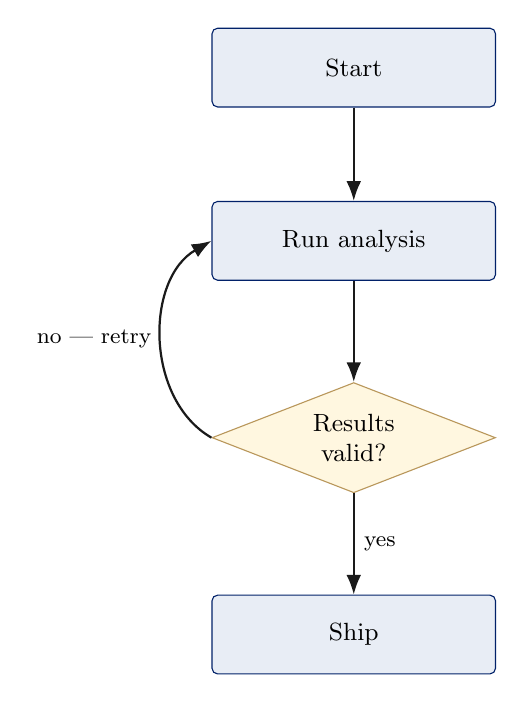
\begin{tikzpicture}
  \node[flow-node]     (start) at (0,  0)   {Start};
  \node[flow-node]     (run)   at (0, -2.2) {Run analysis};
  \node[flow-decision] (check) at (0, -4.7) {Results\\valid?};
  \node[flow-node]     (end)   at (0, -7.2) {Ship};

  \draw[flow-edge] (start) -- (run);
  \draw[flow-edge] (run)   -- (check);
  \draw[flow-edge] (check) -- node[midway, right] {\footnotesize yes} (end);

  % Retry arc — bends out to the left and returns to run
  \draw[flow-edge] (check.west) to[bend left=60]
    node[midway, left] {\footnotesize no — retry} (run.west);
\end{tikzpicture}
\end{document}
